\chapter{Lecture 11: Rindler Horizons and the Schwarzschild Metric}

\lectureoverview{Topology, curvature, and coordinates are easy to
confuse, so they must first be kept separate.  Gauss--Bonnet
fixes the total curvature of a closed surface from its number of
handles, yet a suitable metric can make a torus flat, and deleting one
point from a sphere allows a flat metric pulled back from the plane.
Normal coordinates then remove the connection at one event without
removing curvature.  With that distinction in hand, proper time becomes
the action for a free particle, its weak-field limit identifies
\(g_{00}\) with the Newtonian potential, and uniformly accelerated
observers provide a flat-spacetime model of a horizon.  Rindler
coordinates make the model exact.  The closing construction uses
spherical symmetry, the Newtonian limit, and Birkhoff's theorem to
introduce the Schwarzschild exterior metric.}

We use the spacetime signature
\begin{equation}
  \eta_{\mu\nu}=\operatorname{diag}(1,-1,-1,-1)
  \label{eq:l11-signature}
\end{equation}
and write \(ds^2=c^2d\tau^2\) for a timelike worldline.  Factors of
\(c\) are retained when they clarify dimensions and suppressed where
the geometry is easier to read in units with \(c=1\).

\section{Topology Fixes Total Curvature}

On the outer rim of an ordinary torus the Gaussian curvature \(K\) is
positive; on the inner rim it is negative.  The two contributions
cancel when integrated over the whole surface.  A deformation into a
coffee-cup shape can move positive and negative curvature from place to
place, but it cannot alter the total.  For a closed orientable surface
\(\Sigma_g\) of genus \(g\), Gauss--Bonnet states
\begin{equation}
  \boxed{\int_{\Sigma_g}K\,dA
  =2\pi\chi(\Sigma_g)
  =4\pi(1-g).}
  \label{eq:l11-gauss-bonnet}
\end{equation}
Thus, after division by \(4\pi\), the sphere has total \(+1\), the
torus has \(0\), a two-handled surface has \(-1\), and a three-handled
surface has \(-2\).

\begin{figure}[tbp]
  \centering
  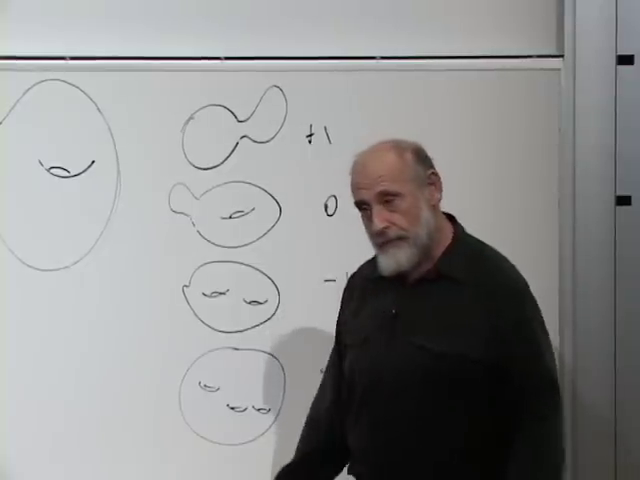
\includegraphics[width=0.82\textwidth]{lecture_11_figure_01.png}
  \caption{The board classification of closed surfaces by handles.  In
  the normalization used in the discussion, their integrated
  curvatures are \(+1,0,-1,-2,\ldots\).}
  \lectureframe{00:03:25}
\end{figure}

The theorem gives an obstruction.  A sphere or a surface with two or
more handles cannot carry an everywhere-flat metric, because
\(K=0\) everywhere would force the integral to vanish.  A torus passes
this necessary test.

\begin{classroomqa}
\audiencequestion{If the torus has zero integrated curvature, does that
prove that the torus already drawn on the board can be unfolded into a
flat sheet?
\lecturetimestamp{00:01:47--00:02:16}}
\lecturerresponse{No.  A zero integral says only that positive and
negative curvature cancel.  It does not force the particular metric to
have \(K=0\) point by point.  Total curvature is a topological
invariant; local curvature still depends on the metric.}
\end{classroomqa}

\begin{classroomqa}
\audiencequestion{Can one nevertheless put an everywhere-flat metric
on a torus?
\lecturetimestamp{00:03:42--00:04:15}}
\lecturerresponse{Yes.  Begin with a Euclidean rectangle and identify
opposite edges.  The quotient is a torus and inherits the flat metric
locally.  It cannot be embedded in ordinary three-dimensional
Euclidean space as the familiar doughnut without bending, but intrinsic
flatness does not require that embedding.}
\end{classroomqa}

This is the first distinction to keep: topology constrains which
metrics are possible, but topology is not itself a metric.

\section{A Sphere with One Point Removed}

Delete the north pole \(N\) from a sphere.  The remaining surface is
topologically a plane.  To see it, rest the sphere on a plane at its
south pole and draw a line from \(N\) through each point \(P\) of the
sphere.  Continue the line until it meets the plane.  This
stereographic projection is one-to-one from \(S^2\setminus\{N\}\) to
\(\mathbb{R}^2\); the missing north pole corresponds to infinity.

\begin{figure}[tbp]
  \centering
  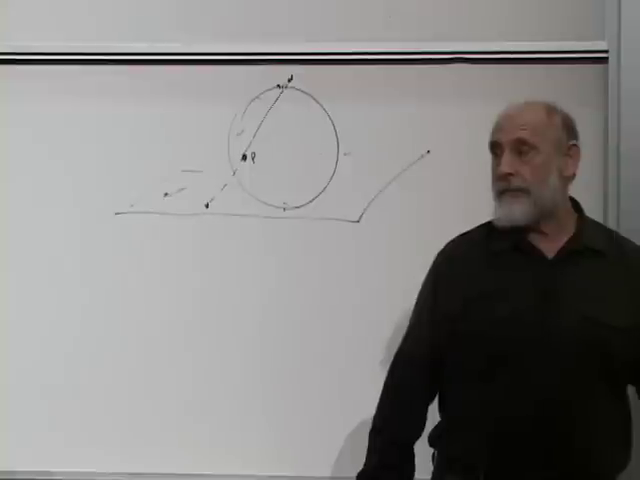
\includegraphics[width=0.82\textwidth]{lecture_11_figure_02.png}
  \caption{Stereographic projection from the deleted north pole onto a
  tangent plane.  Points approaching the deleted pole are sent to
  arbitrarily large distance.}
  \lectureframe{00:07:48}
\end{figure}

Now place the ordinary Euclidean metric
\begin{equation}
  d\ell^2=du^2+dv^2
  \label{eq:l11-plane-metric}
\end{equation}
on the plane and pull it back through the projection.  The resulting
metric on the punctured sphere is flat.  It is not the standard round
metric.  In coordinates that remain finite on the drawn sphere, its
components diverge near \(N\), because a short visual displacement
there represents a very large Euclidean displacement in the plane.
Measuring rods adapted to this metric shrink as they approach the
missing point, and geodesic triangles have angle sum \(180^\circ\).

\begin{classroomqa}
\audiencequestion{Does removing one point really let the sphere become
flat, and what becomes singular?
\lecturetimestamp{00:04:17--00:07:55}}
\lecturerresponse{The punctured surface can be assigned the metric
pulled back from the plane, so its Gaussian curvature is zero
everywhere that remains.  The deleted point lies at infinite distance
in that metric.  What diverges near it are coordinate components of
the pulled-back metric, not the intrinsic curvature on the punctured
surface.}
\end{classroomqa}

\begin{classroomqa}
\audiencequestion{Are the geodesics of this flat metric still great
circles of the round sphere?
\lecturetimestamp{00:07:55--00:08:25}}
\lecturerresponse{In general, no.  Geodesics are determined by the
chosen metric.  Here they are inverse images of straight lines in the
plane.  Under stereographic projection those inverse images are
circles through the deleted north pole, with a limiting straight-line
case, rather than arbitrary great circles of the round metric.}
\end{classroomqa}

\begin{classroomqa}
\audiencequestion{Does this kind of two-variable mapping suggest a
direct physical application?
\lecturetimestamp{00:08:25--00:08:58}}
\lecturerresponse{No immediate example is identified.  The question is
left open rather than used to infer a physical claim, and the
discussion moves to what mappings between different dimensions can
mean mathematically.}
\end{classroomqa}

\subsection{Why cardinality is not a coordinate transformation}

The projection prompts a broader question: can spaces of different
dimension be put into one-to-one correspondence?  As sets, the answer
can be yes.  For \(x,y\in(0,1)\), choose decimal expansions that do not
end in an infinite string of nines,
\[
  x=0.x_1x_2x_3\ldots,\qquad
  y=0.y_1y_2y_3\ldots,
\]
and interleave their digits:
\begin{equation}
  F(x,y)=0.x_1y_1x_2y_2x_3y_3\ldots.
  \label{eq:l11-digit-map}
\end{equation}
The alternating digits can be separated again, so this construction
encodes a pair of real numbers in one real number.  The convention on
terminating expansions removes the familiar ambiguity
\(0.5000\ldots=0.4999\ldots\).

\begin{figure}[tbp]
  \centering
  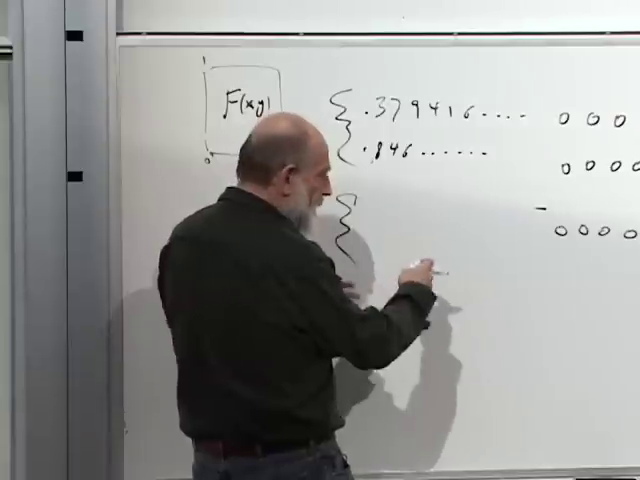
\includegraphics[width=0.88\textwidth]{lecture_11_figure_03.png}
  \caption{The digit-interleaving construction used to compare the
  cardinality of a square with that of an interval.}
  \lectureframe{00:14:48}
\end{figure}

\begin{classroomqa}
\audiencequestion{If two coordinates can be encoded in one number, why
can this not serve as a change of coordinates?
\lecturetimestamp{00:08:58--00:15:40}}
\lecturerresponse{Because a coordinate transformation in geometry must
at least be continuous, and for tensor calculus it must be
differentiable with a nonsingular Jacobian.  Digit interleaving has
none of those properties.  Infinitesimally close points can be sent far
apart, and a smooth function of \(x\) and \(y\) becomes violently
irregular as a function of \(F\).  Equality of cardinality does not
preserve dimension, neighborhoods, or geometry.}
\end{classroomqa}

\section{Normal Coordinates Remove the Connection, Not Curvature}

At any event \(P\), geodesic or Riemann normal coordinates can be chosen
so that
\begin{equation}
  g_{\mu\nu}(P)=\eta_{\mu\nu},
  \qquad
  \partial_\alpha g_{\mu\nu}(P)=0,
  \qquad
  \Gamma^\rho_{\mu\nu}(P)=0.
  \label{eq:l11-normal-coordinates}
\end{equation}
This is the precise local content of freely falling coordinates.  It
does not imply that the derivatives of the connection vanish.  Since
\[
  \Gamma\sim g^{-1}\partial g,
\]
one has schematically
\begin{equation}
  R\sim\partial\Gamma+\Gamma\Gamma
   \sim \partial^2g+(\partial g)^2.
  \label{eq:l11-curvature-schematic}
\end{equation}
At \(P\), the quadratic term vanishes in normal coordinates while the
second-derivative term generally survives.

For example, with the convention
\[
R^\rho{}_{\sigma\mu\nu}
=\partial_\mu\Gamma^\rho_{\nu\sigma}
-\partial_\nu\Gamma^\rho_{\mu\sigma}+\cdots,
\]
the lowered tensor at \(P\) is a linear combination of second metric
derivatives,
\begin{equation}
  R_{\alpha\beta\gamma\delta}(P)
  =
  \frac12\left(
  g_{\alpha\delta,\beta\gamma}
  g_{\beta\gamma,\alpha\delta}
  -g_{\alpha\gamma,\beta\delta}
  -g_{\beta\delta,\alpha\gamma}
  \right)_P.
  \label{eq:l11-riemann-normal}
\end{equation}

\begin{figure}[tbp]
  \centering
  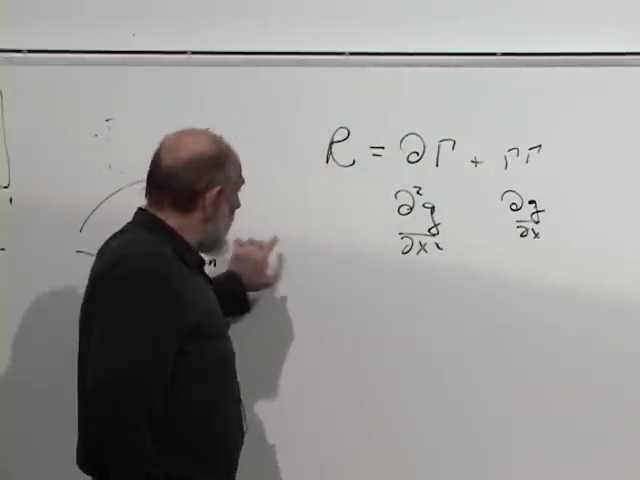
\includegraphics[width=0.82\textwidth]{lecture_11_figure_04.png}
  \caption{The board isolates curvature as
  \(\partial\Gamma+\Gamma\Gamma\), and therefore as second derivatives
  of the metric after first derivatives have been removed at one
  event.}
  \lectureframe{00:19:35}
\end{figure}

\begin{classroomqa}
\audiencequestion{If the metric is Minkowskian and the connection
vanishes at \(P\), how can curvature remain there?
\lecturetimestamp{00:15:42--00:19:55}}
\lecturerresponse{The coordinate choice fixes the value and first
derivatives of the metric at one event, not its second derivatives.
Curvature measures precisely the obstruction that remains at that
order.  One can remove a gravitational field locally in the sense of
free fall, but one cannot transform away tidal effects in a genuinely
curved spacetime.}
\end{classroomqa}

\section{Geodesics and the Proper-Time Action}

A geodesic is defined by parallel transport of its tangent:
\begin{equation}
  u^\nu\nabla_\nu u^\mu=0,
  \qquad
  u^\mu=\frac{dx^\mu}{d\tau}.
  \label{eq:l11-geodesic-covariant}
\end{equation}
In affine coordinates this becomes
\begin{equation}
  \frac{d^2x^\mu}{d\tau^2}
  +\Gamma^\mu_{\alpha\beta}
   \frac{dx^\alpha}{d\tau}
   \frac{dx^\beta}{d\tau}=0.
  \label{eq:l11-geodesic}
\end{equation}
The variational description is local.  A timelike geodesic locally
maximizes proper time among nearby timelike curves, up to conjugate
points.  A Riemannian geodesic is a stationary curve.  A sufficiently
short segment locally minimizes length, but a longer segment may lose
that property after conjugate points and become a saddle; it need not
be the global shortest route.

\begin{classroomqa}
\audiencequestion{Is a geodesic always the shortest path, or in
spacetime always the longest elapsed time?
\lecturetimestamp{00:20:03--00:22:08}}
\lecturerresponse{The invariant statement is stationarity under small
variations.  Timelike geodesics locally maximize proper time over a
suitable interval.  In a positive-definite metric a sufficiently short
geodesic segment is a local length minimum.  A longer geodesic can
become unstable or saddle-like; global claims require additional
conditions and can fail when several geodesics join the same points.}
\end{classroomqa}

Imagine two points on opposite sides of a symmetric hill.  A taut
string can settle along either side, giving two locally stable
geodesics.  A perfectly centered path over the summit is also
stationary.  Within the smooth family pictured on the board it sits at
the top of the route-length comparison, but under unrestricted path
variations it is safer to call it unstable: the smallest lateral
displacement makes it slide to one side.

\begin{figure}[tbp]
  \centering
  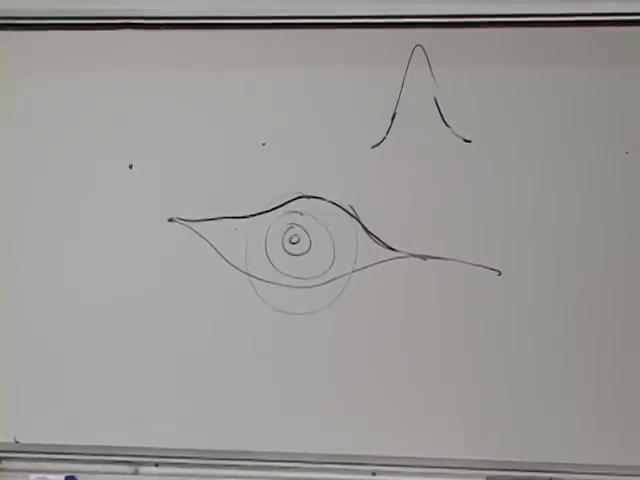
\includegraphics[width=0.82\textwidth]{lecture_11_figure_05.png}
  \caption{Three stationary paths around a hill: two stable routes
  around the sides and one unstable route over the summit.}
  \lectureframe{00:23:55}
\end{figure}

\begin{classroomqa}
\audiencequestion{Can more than one geodesic connect the same two
points, and can one of them be unstable?
\lecturetimestamp{00:22:09--00:25:14}}
\lecturerresponse{Yes.  The hill supplies exactly that example.
Geodesic means stationary, not unique and not necessarily stable.  The
summit path satisfies the geodesic equation even though nearby paths
can be shorter; unrestricted variations also show why stationarity
should not be confused with a global maximum or minimum.}
\end{classroomqa}

For a free massive particle the action is proper time,
\begin{equation}
  S=-mc^2\int d\tau
    =-mc\int ds.
  \label{eq:l11-particle-action}
\end{equation}
Stationarity of this action gives Eq.~\eqref{eq:l11-geodesic}.  Thus
free fall, stationary proper time, and the usual least-action
machinery are three descriptions of the same motion.

\begin{classroomqa}
\audiencequestion{Is the proper-time principle different from the
ordinary principle of least action?
\lecturetimestamp{00:25:14--00:27:10}}
\lecturerresponse{No.  Proper time supplies the Lagrangian for a free
relativistic particle.  Applying the Euler--Lagrange equations to that
action yields the geodesic equation in any metric.}
\end{classroomqa}

\subsection{Using coordinate time}

Take \(x^0=ct\) and define \(v^i=dx^i/dt\).  The line element is
\begin{equation}
  c^2d\tau^2
  =
  g_{00}c^2dt^2
  +2g_{0i}c\,dt\,dx^i
  +g_{ij}dx^i dx^j.
  \label{eq:l11-time-split}
\end{equation}
Therefore
\begin{equation}
  S=\int L\,dt,
  \qquad
  L=-mc^2
  \sqrt{
  g_{00}
  +\frac{2g_{0i}v^i}{c}
  +\frac{g_{ij}v^i v^j}{c^2}}.
  \label{eq:l11-coordinate-lagrangian}
\end{equation}

\begin{figure}[tbp]
  \centering
  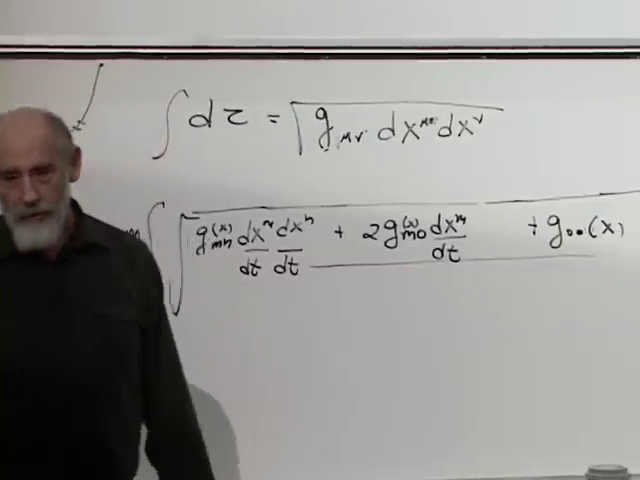
\includegraphics[width=0.92\textwidth]{lecture_11_figure_06.png}
  \caption{The proper-time action rewritten as a coordinate-time
  Lagrangian with the \(g_{00}\), \(g_{0i}\), and \(g_{ij}\) terms
  visible inside the square root.}
  \lectureframe{00:31:48}
\end{figure}

\begin{classroomqa}
\audiencequestion{Why does the mixed \(g_{0i}\) term carry a factor of
two?
\lecturetimestamp{00:29:09--00:29:23}}
\lecturerresponse{Because the symmetric quadratic form contains both
\(g_{0i}\,dx^0dx^i\) and \(g_{i0}\,dx^idx^0\).  Metric symmetry makes
them equal, so together they give \(2g_{0i}\,dx^0dx^i\).}
\end{classroomqa}

The Euler--Lagrange equations derived with \(t\) are equivalent to the
geodesic equation, but \(t\) is generally not an affine parameter.
Changing from \(\tau\) to \(t\) uses
\[
  \frac{d}{d\tau}
  =\frac{dt}{d\tau}\frac{d}{dt}
\]
and introduces a term proportional to \(dx^\mu/dt\):
\begin{equation}
  \frac{d^2x^\mu}{dt^2}
  +\Gamma^\mu_{\alpha\beta}
  \frac{dx^\alpha}{dt}\frac{dx^\beta}{dt}
  =f(t)\frac{dx^\mu}{dt}.
  \label{eq:l11-nonaffine-geodesic}
\end{equation}
The function \(f\) records only the nonaffine parametrization, not a
new force.

\begin{figure}[tbp]
  \centering
  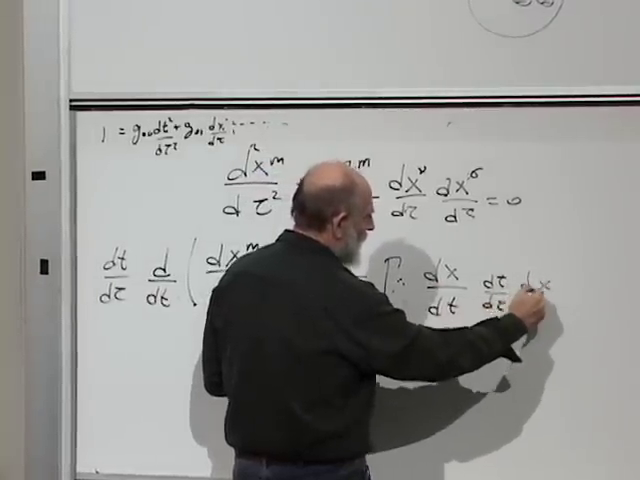
\includegraphics[width=0.88\textwidth]{lecture_11_figure_07.png}
  \caption{The board conversion between derivatives with respect to
  proper time and coordinate time in the geodesic equation.}
  \lectureframe{00:36:02}
\end{figure}

\begin{classroomqa}
\audiencequestion{Why not compare the Euler--Lagrange equation and the
geodesic equation term by term immediately?
\lecturetimestamp{00:32:26--00:36:37}}
\lecturerresponse{They initially use different parameters.  The
standard geodesic equation uses affine proper time, while the displayed
Lagrangian uses coordinate time.  After the chain-rule conversion the
two descriptions agree; carrying every algebraic term adds length but
no new principle.}
\end{classroomqa}

\section{The Newtonian Limit Lives in
\texorpdfstring{\(g_{00}\)}{g00}}

Assume a static weak field, no appreciable mixed components, and slow
motion:
\begin{equation}
  g_{00}=1+h_{00},
  \qquad
  g_{0i}=0,
  \qquad
  g_{ij}\simeq-\delta_{ij},
  \qquad
  |h_{00}|\ll1,\quad v\ll c.
  \label{eq:l11-weak-metric}
\end{equation}
Then Eq.~\eqref{eq:l11-coordinate-lagrangian} becomes
\[
  L=-mc^2
  \sqrt{1+h_{00}-\frac{v^2}{c^2}}.
\]
Using \(\sqrt{1+\epsilon}\simeq1+\epsilon/2\),
\begin{equation}
  L\simeq
  -mc^2
  \frac12mv^2
  -\frac12mc^2h_{00}.
  \label{eq:l11-weak-lagrangian}
\end{equation}
The first term is an irrelevant constant for the equations of motion.
Comparison with
\[
  L_{\mathrm N}=\frac12mv^2-m\Phi
\]
gives
\begin{equation}
  \boxed{
  h_{00}=\frac{2\Phi}{c^2},
  \qquad
  g_{00}\simeq1+\frac{2\Phi}{c^2}.}
  \label{eq:l11-g00-potential}
\end{equation}

\begin{figure}[tbp]
  \centering
  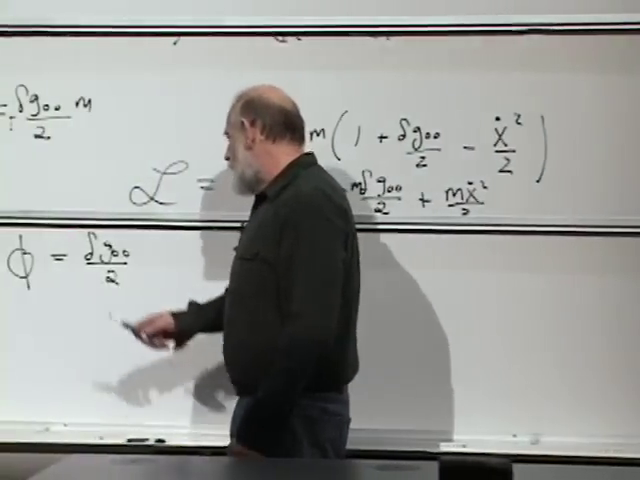
\includegraphics[width=0.88\textwidth]{lecture_11_figure_08.png}
  \caption{The weak-field square-root expansion and its comparison
  with kinetic minus potential energy.}
  \lectureframe{00:43:35}
\end{figure}

\begin{classroomqa}
\audiencequestion{Why is the flat spatial contribution negative in the
square root?
\lecturetimestamp{00:37:04--00:37:44}}
\lecturerresponse{That is the declared Lorentzian signature.  In flat
spacetime \(g_{00}=1\) and \(g_{ij}=-\delta_{ij}\), so
\(c^2d\tau^2=c^2dt^2-d\boldsymbol{x}^2\).}
\end{classroomqa}

\begin{classroomqa}
\audiencequestion{Is the gravitational potential literally
\(g_{00}\)?
\lecturetimestamp{00:39:30--00:43:46}}
\lecturerresponse{No.  The potential is the small departure of
\(g_{00}\) from its asymptotic constant, with
\(h_{00}=2\Phi/c^2\).  Adding a constant to \(\Phi\) corresponds to a
normalization of time and does not alter the Newtonian force.}
\end{classroomqa}

\section{Uniform Acceleration in Special Relativity}

We now approach black holes indirectly.  A Newtonian trajectory with
constant coordinate acceleration,
\[
  X(T)=X_0+V_0T+\frac12aT^2,
\]
eventually has \(|dX/dT|>c\), so it cannot describe uniform
acceleration for all time in special relativity.  Constant
\emph{proper} acceleration instead traces the hyperbola
\begin{equation}
  X^2-c^2T^2=\rho^2.
  \label{eq:l11-acceleration-hyperbola}
\end{equation}
Its asymptotes are the null lines \(X=\pm cT\).  A Lorentz boost moves
a point along the same hyperbola, just as an ordinary rotation moves a
point around a circle.

\begin{figure}[tbp]
  \centering
  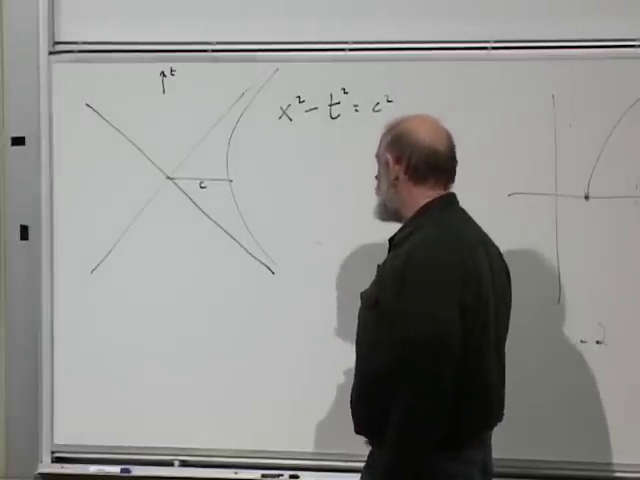
\includegraphics[width=0.82\textwidth]{lecture_11_figure_09.png}
  \caption{A uniformly accelerated worldline as a hyperbola inside
  its light-cone asymptotes, contrasted on the board with the
  Newtonian parabola.}
  \lectureframe{00:49:40}
\end{figure}

\begin{classroomqa}
\audiencequestion{Why is the relativistic uniformly accelerated path a
hyperbola rather than the familiar parabola?
\lecturetimestamp{00:47:24--00:52:22}}
\lecturerresponse{Uniformity refers to acceleration measured in the
instantaneous rest frame.  The invariant hyperbola preserves that
proper acceleration under boosts, while its coordinate speed
approaches \(c\) without exceeding it.  The Newtonian parabola has no
such speed limit.}
\end{classroomqa}

Parameterize the hyperbola by a dimensionless rapidity \(\eta\):
\begin{equation}
  X=\rho\cosh\eta,
  \qquad
  cT=\rho\sinh\eta.
  \label{eq:l11-rindler-transform}
\end{equation}
Along \(\rho=\text{constant}\),
\[
  d\tau=\frac{\rho}{c}\,d\eta,
  \qquad
  a(\rho)=\frac{c^2}{\rho}.
\]
A family of constant-\(\rho\) hyperbolae forms a congruence of
accelerated observers.  Lines of constant \(\eta\) are their successive
surfaces of simultaneity.

\begin{figure}[tbp]
  \centering
  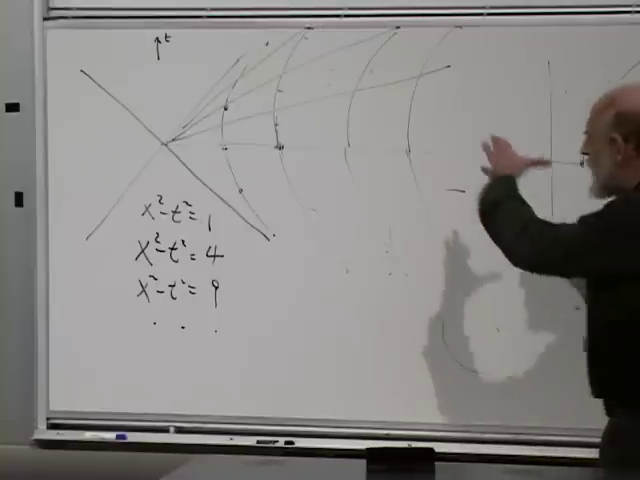
\includegraphics[width=0.84\textwidth]{lecture_11_figure_10.png}
  \caption{A Rindler congruence: constant-\(\rho\) hyperbolae and
  tilted surfaces of constant rapidity inside the right wedge.}
  \lectureframe{00:54:58}
\end{figure}

\begin{classroomqa}
\audiencequestion{Do all observers in a uniformly accelerated frame
feel the same proper acceleration?
\lecturetimestamp{00:55:22--00:58:30}}
\lecturerresponse{No.  A Born-rigid family requires
\(a(\rho)=c^2/\rho\).  Observers nearer the null boundary accelerate
more strongly.  Simply translating one hyperbola to make equal
accelerations would not preserve the proper separation of the
observers.}
\end{classroomqa}

\begin{figure}[tbp]
  \centering
  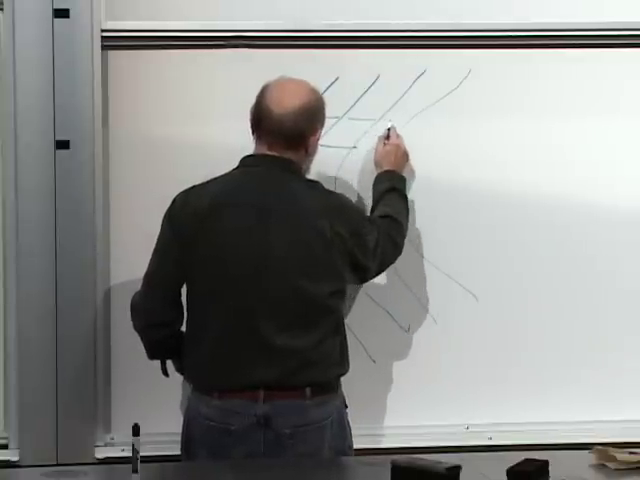
\includegraphics[width=0.82\textwidth]{lecture_11_figure_11.png}
  \caption{The acceleration gradient across the congruence.  The
  hyperbolae crowd toward the null boundary, where the required proper
  acceleration diverges.}
  \lectureframe{00:58:12}
\end{figure}

The equivalence principle lets the accelerated observers describe
their experience as a static gravitational field.  Near a chosen
worldline \(\rho=\rho_0\), put \(\rho=\rho_0+z\) and define local time
\(ct_0=\rho_0\eta\).  The Rindler lapse then gives
\[
  g_{00}=\left(1+\frac{z}{\rho_0}\right)^2
  \simeq1+\frac{2z}{\rho_0}.
\]
Equation~\eqref{eq:l11-g00-potential} identifies
\[
  \Phi\simeq\frac{c^2z}{\rho_0}=a_0z,
  \qquad a_0=\frac{c^2}{\rho_0}.
\]
The effective field strengthens toward smaller \(\rho\).  Nothing in
the underlying spacetime is singular; the noninertial observers are
using rockets in flat Minkowski space.

\section{A Horizon Without Curvature}

Release a rock from one accelerated observer.  The rock ceases to fire
its rocket and follows an inertial straight line in the Minkowski
diagram.  The accelerated congruence bends away from that line, so its
members describe the rock as falling toward \(\rho=0\).

\begin{figure}[tbp]
  \centering
  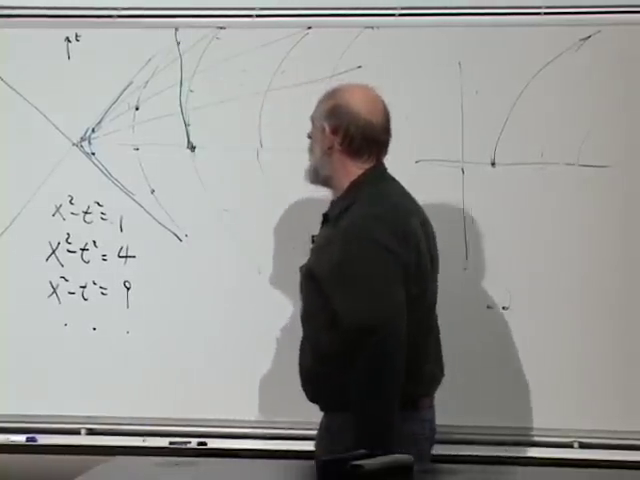
\includegraphics[width=0.84\textwidth]{lecture_11_figure_12.png}
  \caption{An inertial rock crosses the accelerated congruence on a
  straight worldline while the Rindler observers follow hyperbolae.}
  \lectureframe{01:02:38}
\end{figure}

\begin{classroomqa}
\audiencequestion{What happens to a rock released from an accelerated
observer?
\lecturetimestamp{01:02:05--01:03:42}}
\lecturerresponse{It follows an ordinary inertial geodesic.  In
Minkowski coordinates nothing pulls it; in the accelerated frame it
falls toward the Rindler horizon.  The two descriptions concern the
same worldline.}
\end{classroomqa}

Imagine that the rock flashes, rings, or broadcasts periodically.
Signals emitted after it crosses the future null line \(X=cT\) cannot
reach any observer who remains forever in the right Rindler wedge.
That null line is the observers' future horizon.  It is a causal
boundary, not a material membrane and not a region of large curvature.

\begin{figure}[tbp]
  \centering
  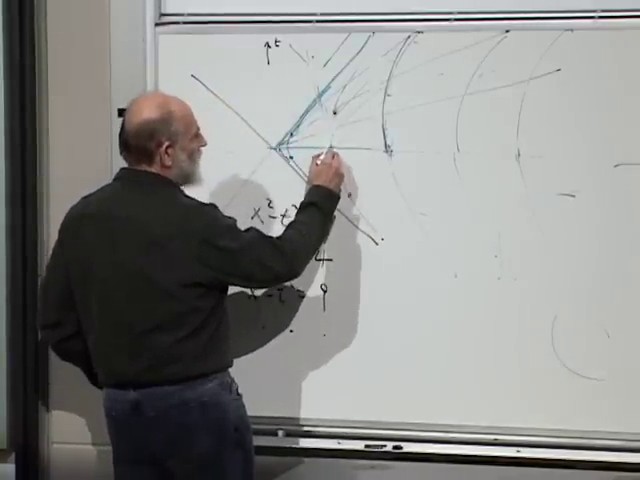
\includegraphics[width=0.84\textwidth]{lecture_11_figure_13.png}
  \caption{Light signals from a released rock and the null boundary
  beyond which they can no longer catch a persistently accelerated
  observer.}
  \lectureframe{01:06:18}
\end{figure}

\begin{classroomqa}
\audiencequestion{Is the horizon an absolute place, and is the
accelerated observer forbidden to cross it?
\lecturetimestamp{01:06:53--01:07:49}}
\lecturerresponse{No.  It is tied to the observer's decision to
accelerate forever.  The observer may switch off the rocket, follow an
inertial path, and cross the same null line.  Different accelerated
worldlines have correspondingly shifted causal boundaries.}
\end{classroomqa}

If a second rock is released later, its inertial path is tangent to the
hyperbola at the later release event.  It too crosses the null
boundary, even though its straight line differs from the first.

\begin{figure}[tbp]
  \centering
  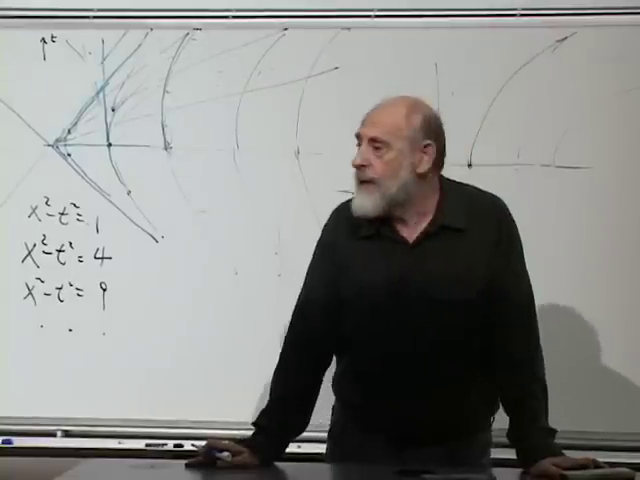
\includegraphics[width=0.84\textwidth]{lecture_11_figure_14.png}
  \caption{A later release produces a different inertial tangent, but
  the same causal lesson: the rock crosses the Rindler horizon while
  accelerated observers remain in the wedge.}
  \lectureframe{01:08:02}
\end{figure}

\begin{classroomqa}
\audiencequestion{Does releasing the rock later prevent it from
crossing the horizon?
\lecturetimestamp{01:07:50--01:08:19}}
\lecturerresponse{No.  The release changes which inertial tangent the
rock follows.  Every such released trajectory can pass through the
future null boundary while the eternally accelerated observers remain
outside it.}
\end{classroomqa}

\begin{classroomqa}
\audiencequestion{After the rock has crossed, can it still receive
signals from the accelerated observers?
\lecturetimestamp{01:08:19--01:09:05}}
\lecturerresponse{Yes.  Future-directed light from outside can cross
inward and reach the rock.  The forbidden direction is outward:
signals emitted by the rock after crossing cannot return to the
eternally accelerated observers.  The horizon is a one-way causal
boundary, not a reflecting wall.}
\end{classroomqa}

\section{Rindler Coordinates}

Equation~\eqref{eq:l11-rindler-transform} is the Lorentzian analogue of
polar coordinates,
\[
  x=r\cos\theta,\qquad y=r\sin\theta.
\]
The circular angle becomes a hyperbolic angle.  The radial coordinate
\(\rho>0\) labels a hyperbola, and \(-\infty<\eta<\infty\) labels the
observer's position along it.  The transverse coordinates \(y,z\)
remain unchanged.

\begin{figure}[tbp]
  \centering
  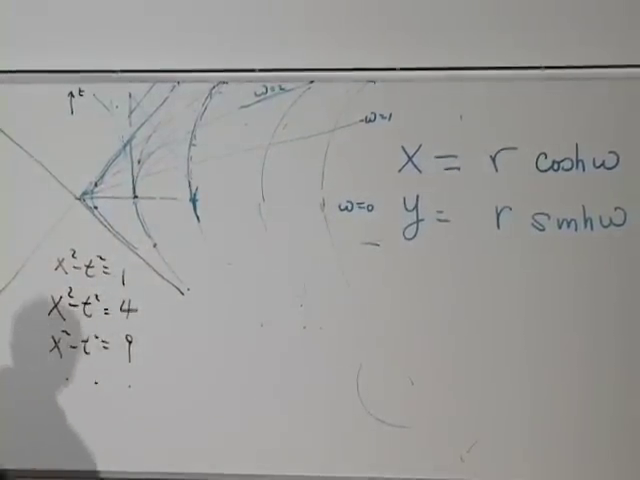
\includegraphics[width=0.9\textwidth]{lecture_11_figure_15.png}
  \caption{Circular polar coordinates beside their hyperbolic
  counterpart \(X=\rho\cosh\eta\), \(cT=\rho\sinh\eta\).}
  \lectureframe{01:13:40}
\end{figure}

Differentiate the transformation:
\begin{align}
  dX&=\cosh\eta\,d\rho
      +\rho\sinh\eta\,d\eta,
      \label{eq:l11-dX}\\
  c\,dT&=\sinh\eta\,d\rho
      +\rho\cosh\eta\,d\eta.
      \label{eq:l11-cdT}
\end{align}

\begin{figure}[tbp]
  \centering
  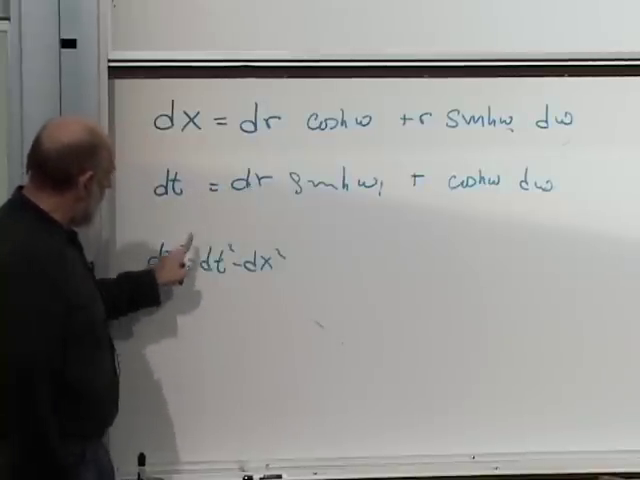
\includegraphics[width=0.9\textwidth]{lecture_11_figure_16.png}
  \caption{The differentiated hyperbolic coordinate transformation
  before substitution into the Minkowski line element.}
  \lectureframe{01:18:50}
\end{figure}

Substitution into
\[
  ds^2=c^2dT^2-dX^2-dy^2-dz^2
\]
cancels the cross terms.  Since
\(\cosh^2\eta-\sinh^2\eta=1\), the result is
\begin{equation}
  \boxed{
  ds^2=\rho^2d\eta^2-d\rho^2-dy^2-dz^2.}
  \label{eq:l11-rindler-metric}
\end{equation}

\begin{figure}[tbp]
  \centering
  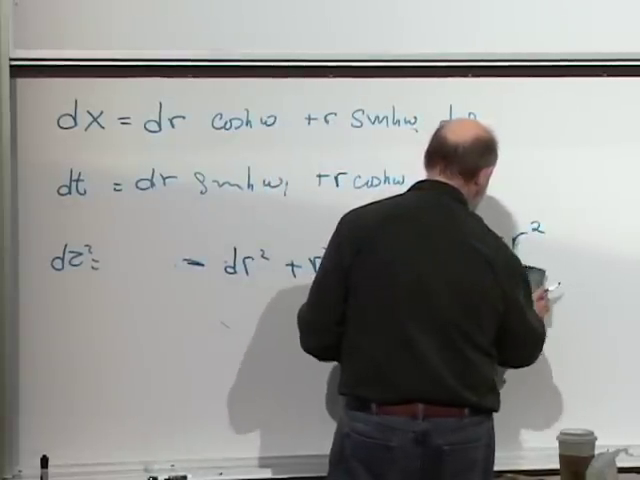
\includegraphics[width=0.9\textwidth]{lecture_11_figure_17.png}
  \caption{The completed Rindler metric.  The coordinate components are
  \(g_{\eta\eta}=\rho^2\) and \(g_{\rho\rho}=-1\), even though the
  underlying spacetime is flat.}
  \lectureframe{01:22:05}
\end{figure}

\begin{classroomqa}
\audiencequestion{Does Rindler space cover all of Minkowski spacetime?
\lecturetimestamp{01:24:03--01:24:20}}
\lecturerresponse{No.  With \(\rho>0\), these coordinates cover only
the right wedge \(X>|cT|\).  The coordinate boundary \(\rho=0\)
corresponds to the two null rays that form the past and future Rindler
horizons.}
\end{classroomqa}

\subsection{An inertial geodesic in accelerated coordinates}

Take the inertial worldline \(X=X_0>0\).  Using
Eq.~\eqref{eq:l11-rindler-transform},
\begin{equation}
  \rho(\eta)=\frac{X_0}{\cosh\eta}.
  \label{eq:l11-rindler-geodesic}
\end{equation}
As \(\eta\to-\infty\), the line enters the wedge through
\(\rho=0\); at \(\eta=0\) it reaches its maximum \(\rho=X_0\); and as
\(\eta\to+\infty\) it returns to \(\rho=0\).  The horizon crossings
occur at finite inertial proper time but at infinite Rindler time.

\begin{figure}[tbp]
  \centering
  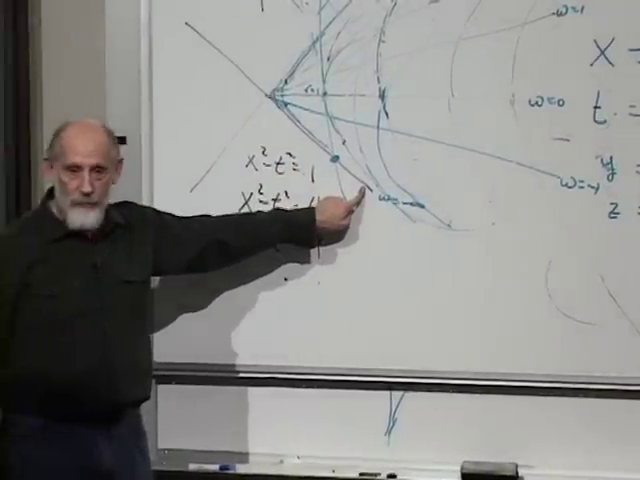
\includegraphics[width=0.9\textwidth]{lecture_11_figure_18.png}
  \caption{The same inertial straight line viewed against the Rindler
  hyperbolae.  In accelerated coordinates it appears to come from the
  past horizon, turn around at maximum \(\rho\), and approach the
  future horizon.}
  \lectureframe{01:27:05}
\end{figure}

\begin{classroomqa}
\audiencequestion{How does a freely falling path look in the
\((\rho,\eta)\) coordinates?
\lecturetimestamp{01:24:22--01:28:32}}
\lecturerresponse{It appears at \(\rho=0\) when
\(\eta=-\infty\), rises to a maximum distance from the horizon, and
returns to \(\rho=0\) when \(\eta=+\infty\).  The infinite coordinate
time is a property of the accelerated clock, not an infinite proper
time for the falling object.}
\end{classroomqa}

Successive pulses from the falling rock take longer to catch the
accelerated observer and arrive increasingly redshifted.  The observer
therefore sees the rock slow and fade near the horizon.  The rock
itself crosses the null line without encountering curvature or a local
singularity.  It can still receive inward signals from the exterior;
their measured frequencies depend on the relative boost and on the
direction of propagation, so one should not replace the causal
statement by a universal redshift or blueshift slogan.

\begin{figure}[tbp]
  \centering
  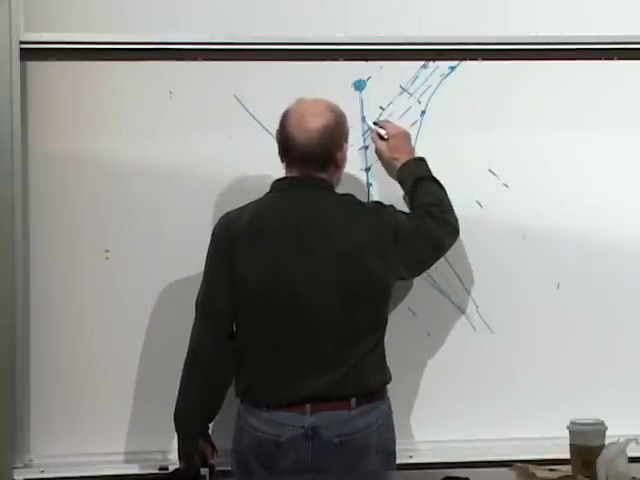
\includegraphics[width=0.84\textwidth]{lecture_11_figure_19.png}
  \caption{The completed causal sketch near the Rindler horizon.  The
  accelerated observer's outgoing view and the infaller's continued
  reception of inward signals are not symmetric.}
  \lectureframe{01:33:55}
\end{figure}

\begin{classroomqa}
\audiencequestion{What does the accelerated observer see, and what
does the falling rock experience at the horizon?
\lecturetimestamp{01:28:33--01:34:20}}
\lecturerresponse{The accelerated observer receives an ever slower,
redder sequence of signals and assigns the crossing to
\(\eta=+\infty\).  The rock crosses in finite proper time and notices
no local singularity.  After crossing it may receive signals sent
inward from the exterior, but it cannot send a causal signal back to
the eternally accelerated observer.}
\end{classroomqa}

\section{Spherical Symmetry and the Exterior Problem}

\begin{samepage}
The Rindler construction required no curvature.  We now turn to a
genuinely gravitating, spherically symmetric source.  The lecture does
not solve the full field equations component by component.  It invokes
the result appropriate to the exterior:

\begin{theorem}[Birkhoff]
Every spherically symmetric solution of the vacuum Einstein equations
with vanishing cosmological constant is locally a member of the
Schwarzschild family.  In particular, the vacuum exterior of a bounded
spherical source is static and depends only on its total mass.
\end{theorem}
\end{samepage}

\begin{classroomqa}
\audiencequestion{Why not write every component of Einstein's equation
and solve the whole system on the board?
\lecturetimestamp{01:34:23--01:37:31}}
\lecturerresponse{Spherical symmetry and the vacuum equations have
already reduced the answer to the Schwarzschild exterior.  A
component-by-component derivation is lengthy and would obscure the
geometric issue the lecture now wants to study: the horizon.  The
time-time coefficient can be motivated from Newtonian gravity; the
radial coefficient is then stated as the field-equation result.}
\end{classroomqa}

Use the standard angular convention: \(\theta\) is polar angle from the
north pole and \(\phi\) is azimuth.  The unit two-sphere has
\begin{equation}
  d\Omega^2=d\theta^2+\sin^2\theta\,d\phi^2.
  \label{eq:l11-unit-sphere}
\end{equation}

\begin{figure}[H]
  \centering
  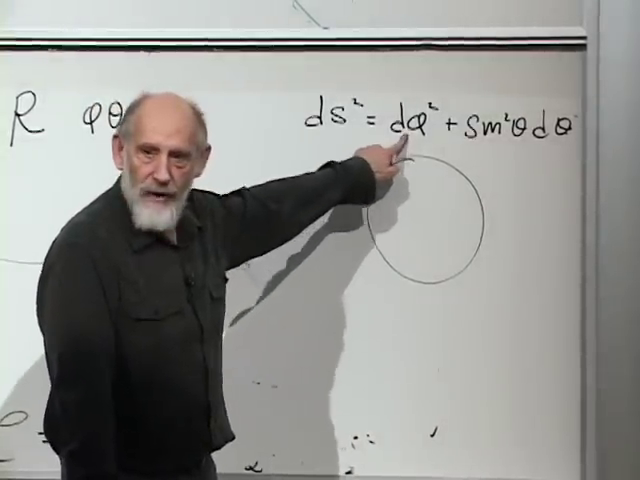
\includegraphics[width=0.84\textwidth]{lecture_11_figure_20.png}
  \caption{The unit-sphere angular element after the live notation is
  normalized to the standard polar angle \(\theta\) and azimuth
  \(\phi\).}
  \lectureframe{01:41:55}
\end{figure}

\begin{classroomqa}
\audiencequestion{Which angular coordinate carries the sine factor?
\lecturetimestamp{01:40:32--01:42:24}}
\lecturerresponse{With the conventional choice used here,
\(\theta\) measures polar angle and \(\phi\) measures azimuth, so
\(d\Omega^2=d\theta^2+\sin^2\theta\,d\phi^2\).  Interchanging the
names is harmless if done consistently; the geometry, not the letter,
is what matters.}
\end{classroomqa}

Flat three-dimensional space in spherical coordinates is
\begin{equation}
  d\ell^2=dr^2+r^2d\Omega^2.
  \label{eq:l11-flat-space-spherical}
\end{equation}
The coordinate \(r\) is the areal radius: every orbit of the rotation
group has area \(4\pi r^2\).

\begin{figure}[tbp]
  \centering
  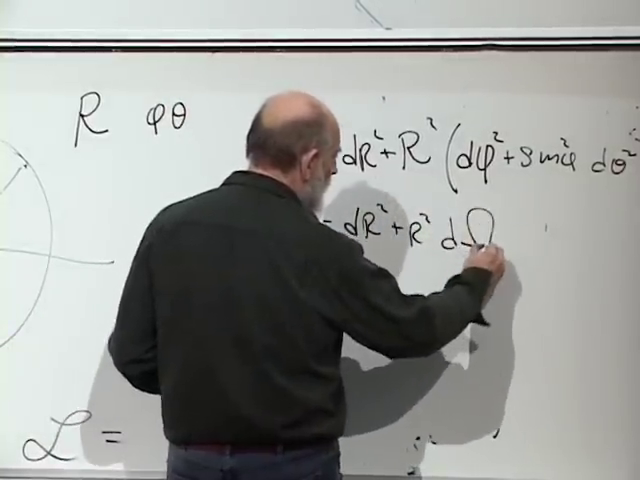
\includegraphics[width=0.88\textwidth]{lecture_11_figure_21.png}
  \caption{The radial and angular pieces of the flat
  three-dimensional line element.}
  \lectureframe{01:44:05}
\end{figure}

Adding time gives the flat spacetime metric
\begin{equation}
  ds^2=c^2dt^2-dr^2-r^2d\Omega^2.
  \label{eq:l11-minkowski-spherical}
\end{equation}

\begin{figure}[tbp]
  \centering
  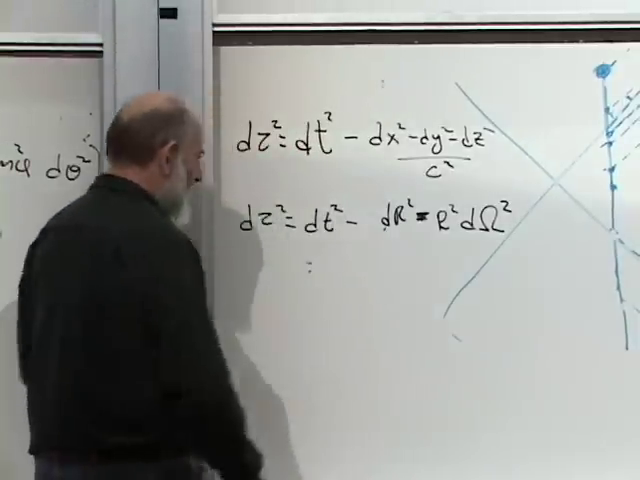
\includegraphics[width=0.88\textwidth]{lecture_11_figure_22.png}
  \caption{Minkowski spacetime written in coordinates adapted to
  spherical symmetry.}
  \lectureframe{01:46:15}
\end{figure}

\section{The Schwarzschild Metric}

Outside a spherical mass \(M\), the Newtonian potential is
\begin{equation}
  \Phi(r)=-\frac{GM}{r}.
  \label{eq:l11-newton-potential}
\end{equation}
The weak-field relation
Eq.~\eqref{eq:l11-g00-potential} then requires
\begin{equation}
  g_{00}\simeq1-\frac{2GM}{c^2r}.
  \label{eq:l11-schwarzschild-g00}
\end{equation}
The constant \(1\) enforces asymptotic flatness.  Far from the source,
the metric approaches Eq.~\eqref{eq:l11-minkowski-spherical}.

\begin{figure}[tbp]
  \centering
  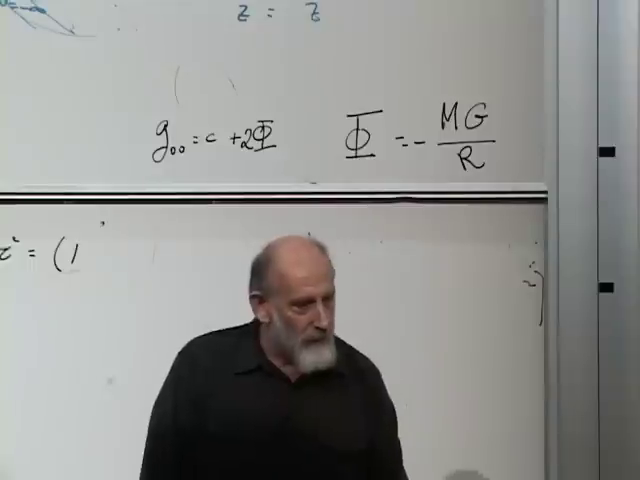
\includegraphics[width=0.88\textwidth]{lecture_11_figure_23.png}
  \caption{The Newtonian potential and the weak-field relation that
  fixes the leading Schwarzschild time component.}
  \lectureframe{01:49:42}
\end{figure}

Define the Schwarzschild radius
\begin{equation}
  r_s=\frac{2GM}{c^2}.
  \label{eq:l11-schwarzschild-radius}
\end{equation}
The exact vacuum exterior metric is
\begin{equation}
  \boxed{
  ds^2=
  \left(1-\frac{r_s}{r}\right)c^2dt^2
  -\frac{dr^2}{1-r_s/r}
  -r^2d\Omega^2.}
  \label{eq:l11-schwarzschild}
\end{equation}

\begin{figure}[tbp]
  \centering
  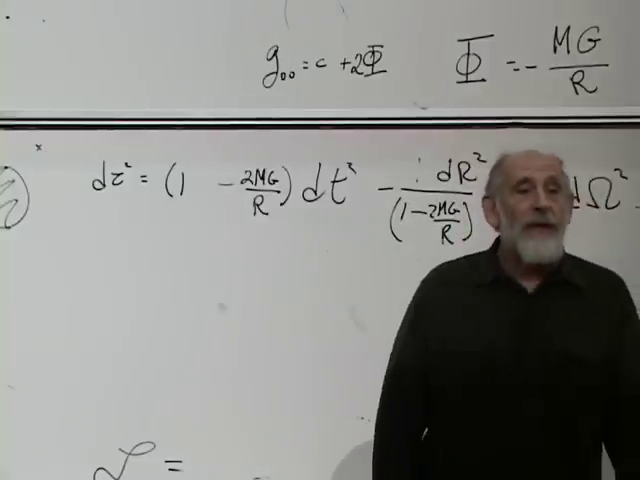
\includegraphics[width=0.92\textwidth]{lecture_11_figure_24.png}
  \caption{The Schwarzschild line element assembled on the board: the
  Newtonian time factor, its reciprocal radial factor, and the
  unchanged areal angular term.}
  \lectureframe{01:53:20}
\end{figure}

The angular coefficient retains the form \(-r^2d\Omega^2\) because
\(r\) has been chosen as areal radius.  This is a coordinate choice,
not a claim that angular geometry is unaffected by gravity.  The
reciprocal factor in the radial term cannot be obtained from the
Newtonian potential alone; it is the additional information supplied
by the vacuum Einstein equations.

Dimensional analysis makes clear why ordinary gravitational fields are
weak.  The expansion parameter is
\begin{equation}
  \frac{GM}{c^2r}=\frac{r_s}{2r}.
  \label{eq:l11-compactness}
\end{equation}
For an ordinary star at radii much larger than \(r_s\), this number is
small.  For a nonrotating, uncharged black hole, the surface
\(r=r_s\) is the horizon.

\begin{figure}[tbp]
  \centering
  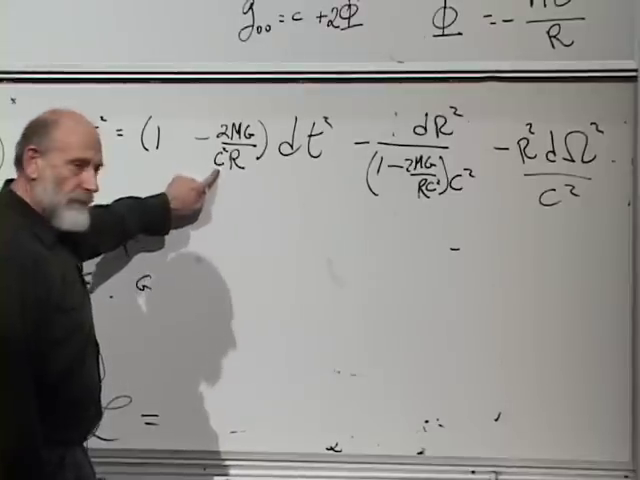
\includegraphics[width=0.84\textwidth]{lecture_11_figure_25.png}
  \caption{The completed Schwarzschild metric with the powers of
  \(c\) restored, making the dimensionless compactness
  \(2GM/(c^2r)\) explicit.}
  \lectureframe{01:56:35}
\end{figure}

At \(r=r_s\), the coefficient of \(dt^2\) vanishes and the coefficient
of \(dr^2\) diverges in Schwarzschild coordinates.  The lecture does
not yet interpret this as a physical singularity.  Its final promise
is instead that, after a suitable near-horizon coordinate
reorganization, the \((t,r)\) part of the geometry will resemble
Rindler space.  The resemblance is hidden by the present coordinates
and will be made explicit next.

\section{From Rindler Space to a Black-Hole Horizon}

Topology fixes integrated curvature, not the local metric.  A torus
admits a flat metric, a punctured sphere admits one pulled back from the
plane, and no discontinuous digit encoding can replace a smooth
coordinate transformation.  Normal coordinates flatten \(g\) and its
first derivatives at one event while leaving second derivatives.

The proper-time action gives free motion, and its weak-field limit
identifies \(g_{00}\simeq1+2\Phi/c^2\).  A family of uniformly
accelerated observers occupies one wedge of flat spacetime and has a
one-way horizon even though the Riemann tensor vanishes.  Schwarzschild
geometry then supplies a curved exterior.  Its horizon looks different
algebraically, but the causal and near-horizon comparison is prepared.
